\chapter{Zpracování dat}

Tato kapitola se zabývá popisem práce s~konkrétní datovou sadou, kterou jsem obdržela. Z~důvodu ochrany dat se v~textu nevyskytují přesná pojmenování, ani není možné zobrazit přesnou strukturu uložení dat. K~dispozici jsem měla data se záznamy za poslední dva roky. 

Z důvodu rozsáhlého množství dat jsem pro analýzu shrinků společnosti vybrala pouze data týkající se měsíce března roku 2023. Všechny analýzy se tak týkají průzkumu shrinku v~tomto období. Tento měsíc se jevil jako vhodný, protože se v~ tomto období nekonaly žádné statní svátky v~České republice, které by narušily chování společnosti a tržní poptávky. Nelze dělat závěry pro chování shrinků během celého roku, neboť mnoho produktů se chová sezónně. Stejně tak poptávka trhu se během delšího časového období mění.  Data týkající se jednoho měsíce obsahují přes milion řádků. Navíc by mohlo vzhledem k~proměnlivosti poptávky během jednoho roku u jednotlivých produktů mnohem obtížnější najít hlavní příčinu shrinku.
% TODO, TBD

\section{Popis obdržených dat}

Všechna data poskytnutá společností jsou uložena v~databázi, ke které byl zhotoven omezený přístup pro účely získání dat pro analýzy shrinku produktů společnosti. Zároveň s~možností přístupu jsem obdržela i tabulku, která stručně komentuje všechny tabulky v~databázi a sloupce v~jednotlivých tabulkách. Celkem se v~databázi nachází přes čtyři sta tabulek, z~nichž bylo potřeba vybrat pouze ty, které obsahují relevantní data pro úlohu shrinků.

S databází jsem pracovala pomocí nástroje \emph{HeidiSQL}, pro získání pouze potřebných dat jsem využívala příkazů jazyka SQL.
Z důvodu ochrany dat nelze uvádět přesné názvy tabulek, nicméně pro lepší orientaci v~textu, každé použité tabulce přiřadím název, který odpovídá obsaženým datům v~tabulce. 

\subsubsection{Číselníky}

Základní číselník s~údaji o produktech, se nachází v~tabulce \emph{produkt} se 27 sloupci. Pro analýzu vzniku shrinků jsem z~této tabulky vybrala jako možné významné údaje následující sloupce:

\begin{itemize}
    \itemsep0em 
    \item \textbf{ID produktu}
    \item \textbf{ID prodejní varianty} -- Určuje o jaký typ balení daného produktu se jedná    
    % \item \textbf{Expirace} -- Expirace produktu ve dnech (hodnoty 0, 999 a NULL označují neomezenou expiraci)
    \item \textbf{ID kategorie} -- Kategorie produktu v~číselné struktuře (pro lepší interpretaci, o jakou kategorii zboží se jedná, je vhodnější použít strukturu podle úrovní, kterou lze získat napojením na tabulku \emph{produkt\_kategorie}.)
    \item \textbf{Aktivní} --  Zda je tento produkt stále aktivní v~portfoliu, nebo se jedná o produkt, který se již neprodává
\end{itemize}

Tabulka \emph{produkt\_kategorie} obsahuje převod z~číselné struktury kategorií do struktury s~produktovou hierarchií. V~obdržených datech má produktová hierarchie šest úrovní. Hierarchie produktů tvoří tedy strom se šesti úrovněmi. Nejvyšší úroveň, tj. úroveň číslo 1 má sedm podkategorií.

V tabulce \ref*{tab:d:4Bzast} jsou uvedeny počty podkategorií pro každou z~kategorií z~nejvyšší, první úrovně. Také je uvedeno procentuální zastoupení kategorií v~nejvyšší úrovni v~rámci produktového portfolia vybrané společnosti. Zastoupení je odvozeno podle počtu produktů v~kategorii.

\begin{table}[hbtp!]
    \captionsetup{justification=centering}
    \begin{center}
    \caption{Počet podkategorií na jednotlivých úrovních a zastoupení \\ nejvyšší kategorie v~rámci produktového portfolia.}
    \label{tab:d:4Bzast}
    \begin{tabular}{rp{4cm}  r r r r r  c}
        & Název kategorie & \multicolumn{5}{c}{Počty kategorií} &      Zastoupení kategorie      \\
        \midrule

        Úroveň: & 1       & 2    & 3   & 4   & 5    & 6    &  \\

        \midrule
        & Nepotravinářské    & 1     & 7    & 27   & 76    & 179   & 76,12\%              \\
        & Suché         & 3     & 13   & 33   & 147   & 494   & 7,28\%               \\
        & Kosmetika a drogerie        & 1     & 4    & 21   & 59    & 193   & 7,07\%               \\
        & Čerstvé       & 5     & 11   & 27   & 111   & 469   & 4,27\%               \\
        & Velmi čerstvé & 6     & 10   & 31   & 92    & 271   & 4,04\%               \\
        & Ostatní     & 4     & 4    & 4    & 5     & 5     & 1,06\%               \\
        & Tabák    & 1     & 1    & 1    & 3     & 8     & 0,17\%   \\
    \end{tabular}
    \end{center}
    \end{table}

Poslední, šestá úroveň hierarchie je přímo napojená na hodnotu číselné struktury, která je uvedena v~číselníku produktů (v tabulce \emph{produkt}). Pro získání všech úrovní kategorizace po úrovních k~danému produktu je třeba vyhledat v~tabulce \emph{produkt} číselné ID kategorie daného produktu a napojit jej na poslední úroveň v~tabulce produktové hierarchie (\emph{produkt\_kategorie}). V~této tabulce je pak uvedena rodičovská kategorie z~úrovně 5. Poté je potřeba opět vyhledat v~tabulce \emph{produkt\_kategorie} tuto hodnotu a zjistit její nadřazenou kategorii. Takto se postupuje dokud není dosaženo nejvyšší úrovně. Tyto operace jsem provedla SQL příkazem přímo nad databází. Použila jsem vnitřní spojení na každou úroveň hierarchii na sloupce kategorie a rodičovská kategorie.

Další tabulka, se kterou jsem pracovala obsahuje informace o velikosti a hmotnosti produktů. Tato tabulka je důležitá z~toho důvodu, že některé položky jsou vážené. Pokud se udává jejich množství, udává se v~gramech, zatímco nevážené položky jsou uvedeny v~kusech. Aby bylo možné porovnávat oba číselné údaje, ke každému váženému produktu existuje přepočet na počet kusů (ozn. SKU). K~tomu jsou využity údaje o počtu kusů na jednu vychystávací jednotku (dále označeno jako $SKU_{\mathrm{VJ}}$) a hmotnost jedné vychystávací jednotky daného produktu (ozn. $m_{\mathrm{VJ}}$). Vychystávací jednotka je jednotka množství používaná pro vychystávání produktů -- jeho balení a transport. Postup pro přepočet hmotnosti produktu na počet kusů ($SKU_{\mathrm{v}}$) je následovný: $$SKU_{\mathrm{v}} = \frac{m}{m_{\mathrm{VJ}}} \cdot SKU_{\mathrm{VJ}},$$
kde $m$ je hmotnost produktu. Ze vzorce vyplývá, že může vyjít neceločíselný počet kusů. Vzhledem k~tomu, že tento přepočet se použije k~porovnávání velikosti objemů, nikoli k~objednávání zboží, tak tato skutečnost není problém.



Číselník prodejen je obsažen v~tabulce \emph{prodejny}. Vybrala jsem z~tabulky následující sloupce. Opět bylo třeba vybrat pouze ty prodejny, které jsou aktivní.
\begin{itemize}
    \itemsep0em 
    \item \textbf{ID prodejny} -- Označení prodejny nebo skladu
    \item \textbf{Název} -- Název prodejny, který obsahuje název města, kde se prodejna nachází.
    \item \textbf{ID kategorie prodejny} -- Do jaké kategorie prodejna nebo sklad patří - zda se jedná o malou nebo velkou prodejnu nebo o sklad. Zavřené prodejny mají hodnotu v~tomto sloupci prázdnou.
\end{itemize}

S číselníkem prodejen souvisí číselník pro jejich zařazení do skupin \emph{prodejny\_skupiny}. Skupiny se mohou v~čase měnit. Pro analýzu jsou relevantní tyto sloupce:
\begin{itemize}
    \itemsep0em 
    \item \textbf{ID prodejny} -- Označení prodejny nebo skladu
    \item \textbf{ID skupiny prodejen} -- Prodejny jsou sdruženy do skupin. Ty se například používají pro hromadné objednávání, nebo pro plánování promoakcí. 
\end{itemize}    

Promoakce se nachází v~tabulce \emph{promoakce}. Z~této tabulky jsou pro následnou analýzu potřebné údaje o ID produktu, počátečním a koncovém datu promoakce a ID skupiny prodejen, na kterých promoakce platí. Promoakce nejsou přiřazené na konkrétní prodejny, ale na skupiny prodejen. Pro další analýzy shrinků je třeba zjistit, zda byl konkrétní zaznamenaný shrink v~době záznamu v~promoakci, nebo ne. Z~tohoto důvodu bylo potřeba tabulky spojit pomocí příkazu \texttt{JOIN} s~číselníkem \emph{prodejny\_skupiny} podle ID prodejny. Z~dat o promoakcích vyplynulo, že pro jeden produkt, může být na dané prodejně v~určité období více promoakcí. V~takovém případě je potřeba vybrat pouze promoakci s~nejvyšší prioritou.

\subsubsection{Tabulky transakcí}
V tabulce \emph{transakce} se nachází údaje o všech provedených transakcích, a to jak skladové transakce, tak prodeje a další pohyby na prodejnách. V~případě prodejů prodejen jsou údaje agregované podle prodejny, konkrétního produktu a dne transakce, tzn. v~této tabulce nelze rozlišit konkrétní prodeje na jednotlivých pokladnách, ale pouze souhrn za jeden den. Tabulka obsahuje údaje za posledních dvanáct měsíců.

Tabulka transakcí obsahuje 21 sloupců, jako možné podstatné sloupce pro analýzu jsem vybrala následující sloupce:

\begin{itemize}
    \itemsep0em
    \item \textbf{ID transakce} -- Jedinečné pro každou transakci.
    \item \textbf{ID produktu} -- Produkt kterého se transakce týká. Každá transakce obsahuje údaje pouze o jediném produktu. 
    \item \textbf{ID prodejny} -- Transakce je takto přiřazená prodejně, případně skladu. % Z~důvodů ochrany dat jsem původní ID převedla na hodnoty od 0 do $p$, kde $p$ je počet prodejen. %TODO TBD (jo chci to tam?)
    \item \textbf{Datum transakce} -- Jedná se o obchodní datum, pokud samotná transakce proběhne až po půlnoci uvedeného dne, tak se posílá s~datem z~předchozího dne, neboť obchodně patří do toho dne.
    \item \textbf{ID promoce} -- Příznak zda a v~jaké promoční akci se produkt nacházel v~čase uvedeném v~datu transakce. V~rámci zpracování dat vyplynulo, že tento příznak není zcela věrohodný 
    \item \textbf{Typ transakce} -- Příznak, zda se jedná např. o prodej, výdej, korekce pohybů a jiné. 
    \item \textbf{ID shrinku} -- Obsahuje označení jednotlivých typů shrinků viz sekce \ref*{sec:shrinkyTypy}. Celkem je identifikováno sedmnáct typů shrinků. V~databázi tento sloupec označuje i jiná ID než ta, která se týkají shrinků, z~toho plyne, že bylo třeba vyfiltrovat pouze ta data, která obsahují sedmnáct identifikačních čísel označující shrinky. V~případě, že typem transakce jsou např. příjmy tento parametr nehraje roli. % Z~důvodu anonymity dat jsem původní ID přečíslovala na celočíselné hodnoty od 0 až do počtu shrinků (pro obě hlavní kategorie). %TODO TBD (jo chci to tam?)
    \item \textbf{Objem} -- Množství produktu uvedené v~transakci. U kusových produktů se jedná o celočíselný údaj u vážených to je desetinné číslo.
    \item Hodnota transakce v~nákladové ceně (desetinné číslo).
    \item Hodnota transakce v~prodejní ceně včetně DPH -- v~případě prodejů se jedná o skutečnou cenu, u zbylých transakcích je uvedena odpovídající cena podle ceníku.
\end{itemize}
Z transakční tabulky je možné získat tabulku se záznamy shrinků a tržeb prodejen. Velikost tabulky se záznamy shrinků za jeden kalendářní rok je přibližně $3.5$ GB.

Tabulku, která obsahuje údaje o jednotlivých, neagregovaných prodejích na prodejnách společnosti, jsem pro účely této práce nazvala \emph{transakce\_prodeje}. Celkem obsahuje třináct sloupců. Tato tabulka je vhodná pro analýzu shrinků typu snížení ceny, analýzou tohoto typu se tato práce nezabývá. Pro ostatní typy, není tato tabulka relevantní. Stejně tak není třeba zkoumat ceník jednotlivých produktů, protože v~souhrnné tabulce transakcí je již uvedená hodnota transakce v~prodejní ceně.

\subsubsection{Další datové zdroje}

Dále jsem pracovala s~daty z~databáze Českého statistického úřadu \cite{bib:czso}. Na webové stránce úřadu je dostupný odkaz ke stažení souboru ve formátu xlsx. Soubor obsahuje údaje o 237 českých městech za posledních několik desítek let. Některá města obsahují záznamy až sto let nazpět, jiné nemají tak dávno zaznamneanou historii. Dataset obsahuje údaje o lokalite, o počtu obyvatel, o sňatcích, rozvodech, stěhování obyvatel a další. V~rámci přípravy dat bylo potřeba napojit prodejny k~údajím o okresu, kraji a počtu obyvatel, kteří žijí v~okolí prodejny. Soubor s~demografickými údaji bylo třeba převést do tabulkové struktury, kde každý řádek patří jednomu městu, protože původní struktura byla nastavená, co list v~souboru, to jedno město. Navíc stejné informace nejsou vždy umístěné stejně na každém listu. 


% \subsection{Období jednoho roku}

% 
Sledovala jsem tři různé veličiny, kterými lze hodnotit transakce - počet záznamů (tj. počet řádků) v tabulce \texttt{transakce}, celkové množství produktů a celková nákladová cena produktů. 

Z databáze jsem vybrala všechny transakce za rok 2022, u kterých byl evidován nějaký typ shrinku. Celkem se jednalo o %doplnit!!!
záznamů. Data jsem agregovala po jednotlivých měsících a pro každý měsíc vypočítala pomocí nástroje pivottables.


typ shrinku v závislosti na expiraci
typ shrinku v závislosti hlavní kategorii produktu
typ shrinku v závislosti na dni v měsíci
typ shrinku v závislosti na dni v týdnu

typ shrinku v závislosti na prodejně, neboli typu prodejny nebo v závislosti na centrálním skladu.
Závislost mezi prodejnami a typem produktu


\subsubsection*{Celkový přehled}

Nejprve jsem určila zastoupení jednotlivých shrinků během celého roku, a to bez uvažování závislosti na jiných faktorech. Poměr rozdělení lze vidět na obrázku \ref*{obr:rok:g:celkemD}.
Největší zastoupení, z pohledu všech tří sledovaných charakteristik, má shrink označující prošlé a zkažené zboží. Z pohledu počtu záznamů činí $70{,}24$ \% ze všech shrinků typu damage, což odpovídá 13 milionům řádkům záznamů. V případě množství neprodaných kusů produktů bylo v roce 2022 odepsáno 40 milionů kusů (tj. $65{,}67$  \%). Podle nejdůležitějšího ukazatele - nákladové ceny - tento shrink měl za následek ztrátu 635 milionů Kč (tj. $57{,}94$) \%.
Další damage shrinky, které mají zastoupení větší než 10  \% je shrink označující poškozené zboží a shrink s produkty, které byly odevzdány potravinové bance.
Zbylé shrinky mají v ročním pohledu malý počet výskytů a jejich výskyt bude analyzován v závislosti na dalších faktorech. 

\begin{figure}[hbtp!]
    \centering
    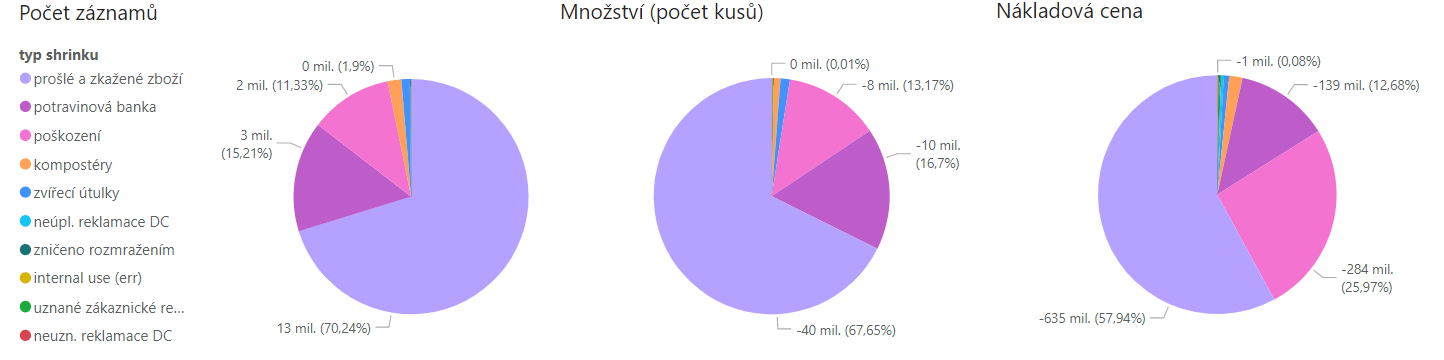
\includegraphics[width=\textwidth]{obrazky/grafy/Graf_celkem-D.png}
    \caption{Zastoupení shrinků typu damage v roce 2022.}
    \label{obr:rok:g:celkemD}
\end{figure}

\subsubsection*{Závislost typu shrinku na čase}

Porovnala jsem množství zaznamenaných shrinků v závislosti na dnech v týdnu, porovnání lze vidět na obr. \ref*{obr:rok:g:tydenD}. Jednotlivé typy jsou zastoupeny analogicky jako v souhrnném přehledu shrinků za jeden rok, tj. prošlé zboží, zboží zaslané do potravinové banky a poškozené zboží. Počty záznamů pro všechny dny jsou v rozmezí $1{,}6$ až $1{,}9$ milionů záznamů  za jeden rok. %!!! nebylo by lepsi tam dat prumer souctu za mesic za cely rok???

\begin{figure}[hbtp!]
    \centering
    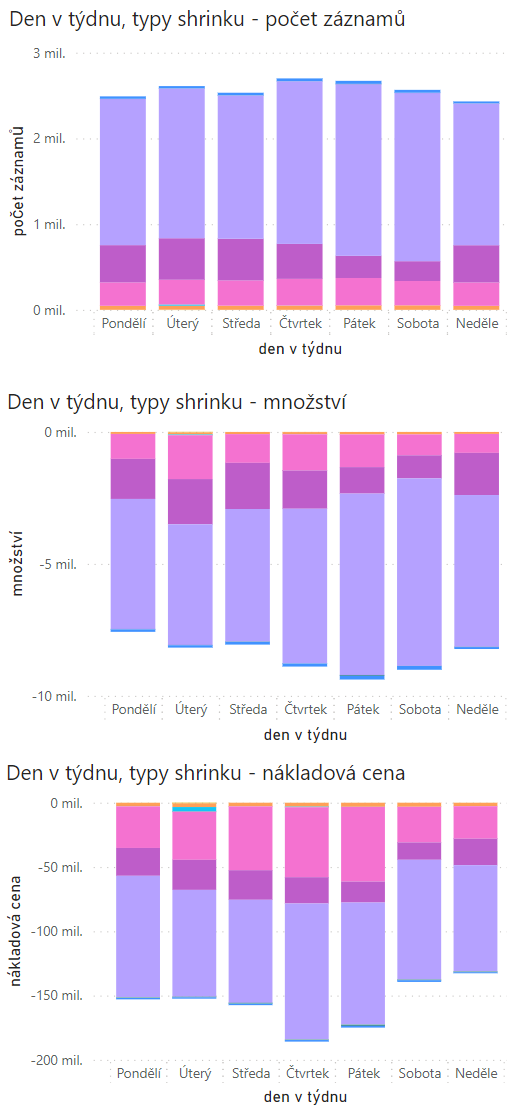
\includegraphics[width=0.5\textwidth]{obrazky/grafy/Grad_dny_tyden-D.png}
    \caption{Zastoupení shrinků typu damage v závislosti na dni v týdnu (údaje pro rok 2022).}
    \label{obr:rok:g:tydenD}
\end{figure}

\begin{figure}[hbtp!]
    \centering
    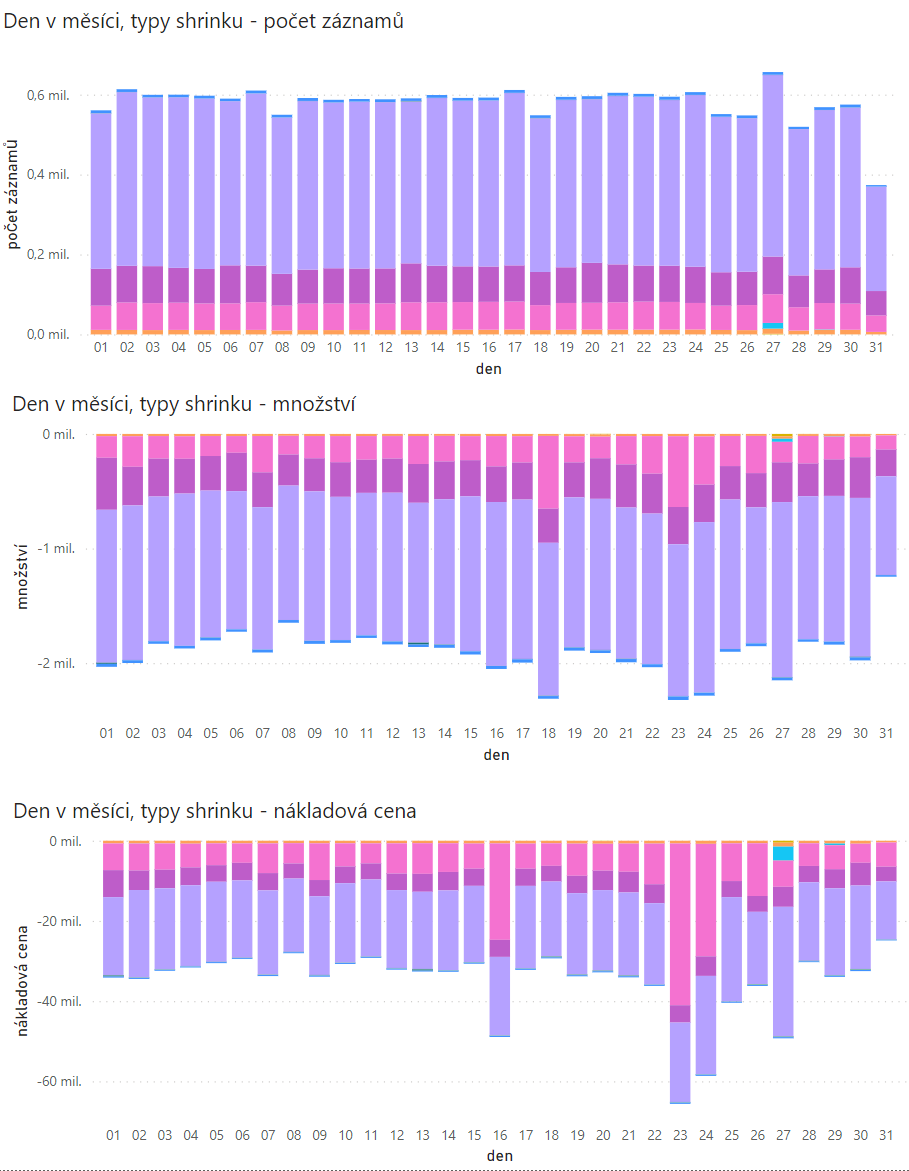
\includegraphics[width=\textwidth]{obrazky/grafy/Grad_dny_mesic-D.png}
    \caption{Zastoupení shrinků typu damage v závislosti na dni v měsíci (údaje pro rok 2022).}
    \label{obr:rok:g:mesicD}
\end{figure}

\subsubsection*{Závislost typu shrinku na hlavní kategorii zboží}

Kategorií, u které bylo evidováno nejvíce damage shrinků je kategorie produktů \emph{superfresh}. V rámci této kategorie je opět nejčastější příčinou odpisu zboží překročená doba expirace, u \emph{superfresh} produktů spíše viditelné zkažení zboží, neboť část \emph{superfresh} produktů nemá uvedenou dobu spotřeby. Druhý nejčastější shrink je shrink označující potravinovou banku. Zbylé shrinky jsou pro tuto kategorii již méně zastoupeny. Kategorie \emph{superfresh} má největší zastoupení většiny typů shrinků nad ostatními kategoriemi - přehled zastoupení jednotlivých shrinků odděleně je na obr. \ref{} %!!! udělat obrazek kde budou vedle sebe grafiký pro kazdy shrink


\subsubsection*{Závislost typu shrinku na typu prodejny}






Vzhledem k vysokému počtu dat pro jeden kalendářní rok, 
v roce 2022 bylo v databázi evidováno přes 32 milionů záznamů o týkající se shrinků
, jsem se rozhodla provést analýzu na měsíčním výběru dat z tohoto období. Jako zkoumaný měsíc jsem vybrala měsíc říjen, neboť v porovnání s letními měsíci a Vánocemi se v říjnu nevyskytují významné sezónní výkyvy.

% [2602933,
%  2439363,
%  2756406,
%  2618723,
%  2809775,
%  2624598,
%  2462898,
%  2545123,
%  2592480,
%  2712669,
%  2543758,
%  2524416]
% 31233142

Zkoumaná říjnová data obsahují $2\ 712\ 669$ řádků a patnáct sloupců. Každý řádek odpovídá jednomu záznamu v databázi shrinku daného produktu. Sledované údaje ve sloupcích jsou: 
% \subsubsection{Sledované údaje}
\begin{itemize}
    \item ID prodejny, kategorická proměnná,
    \item ID produktu, kategorická proměnná,
    \item datum transakce, kategorická proměnná,
    \item typ shrinku, kategorická proměnná,
    \item L1, kategorická proměnná,
    \item L2, kategorická proměnná,
    \item L4, kategorická proměnná,
    \item L5, kategorická proměnná,
    \item L6, kategorická proměnná,
    \item expirace, kategorická proměnná,
    \item množství, spojitá proměnná,
    \item ztracená nákladová cena, spojitá proměnná,
    \item den v týdnu, kategorická proměnná,
    \item číslo den, kategorická proměnná,
    \item období v měsíci (rozdělení měsíce na pět částí), kategorická proměnná.
\end{itemize}
Původní sloupec datum jsem rozdělila na tři jiné proměnné, a to den v týdnu, číslo dne a období v měsíci a sloupec datum jsem vynechala. Z důvodu vysokého počtu záznamů a odlišné povahy dvou typů shrinků jsem data dále rozdělila na shrinky typu damages a shrinky typu inventory. 


\subsection*{Damages shrinky}
Následující část text bude věnována rozboru dat pro shrinky typu damages.



\subsubsection{Výběr dat}
% výběr dle zastoupení shrinků a kategorií produktů a dle outlierů.

Nejprve jsem graficky analyzovala zastoupení shrinků v závislosti na vybraných proměnných pomocí nástroje Power BI, viz obr. \ref*{obr:rok:g:zastoupeni1}. V návaznosti na zjištěné zastoupení shrinků v datech jsem se rozhodla vybrat pouze ty typy shrinků, které tvoří více jak jedno procento z celkových nákladů (tj. náklady činily alespoň jeden milion korun). Vynechala jsem tedy shrinky s označením 5 až 9 a naopak shrinky 0 až 4 byly ponechány. Obdobně jsem přistupovala k záznamům i z hlediska kategorie produktu úrovně L1, jelikož z grafu je patrné, že majoritní zastoupení mají pouze dvě kategorie, a to kategorie superfresh a fresh produktů. Všechny záznamy se zbylými kategoriemi (HBC, others, nonfood, dry food a tobacco) jsem z datasetu odstranila. Těmito kroky jsem zredukovala původní počet řádků datasetu na $1\ 393\ 223$ řádků.

\begin{figure}[hbtp!]
    \centering
    \captionsetup{justification=centering}
    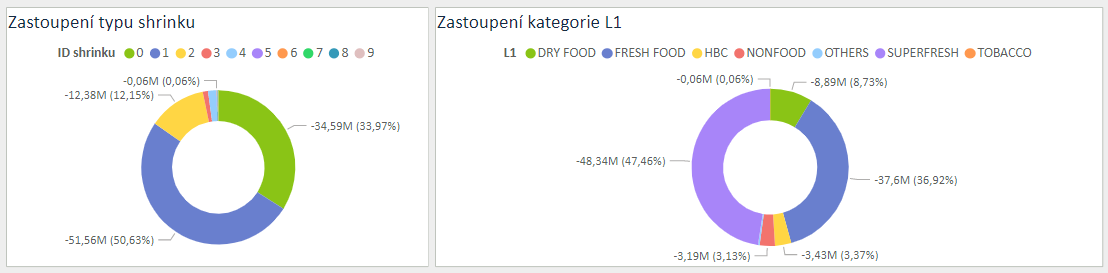
\includegraphics[width=\textwidth]{obrazky/grafy/zastoupeni1.png}
    \caption{Zastoupení shrinků typu damage a zastoupení kategorie L1 v datech \\ z října roku 2022.}
    \label{obr:rok:g:zastoupeni1}
\end{figure}

Jako cílové sloupce (\emph{target} sloupce) jsem určila sloupec s typem shrinku, množstvím produktu a nákladovou cenou. Zbylých jedenáct sloupců slouží jako vysvětlující pro-\linebreak měnné, dále budou označovány jako příznaky pro cílový sloupec. Všechny vybrané příznaky jsou kategorické proměnné, které lze dále rozdělit na nominální a ordinální. Nominální proměnné jsou ID prodejny, ID produktu, kategorie L1, L2, L4, L5 a L6. Ordinální proměnné jsou expirace, den v týdnu, číslo dne a období měsíce. Ordinální příznaky jsem přeznačila tak, aby každá obsahovala pouze hodnoty od nuly do $n_p$, kde $n_p$ je počet kategorií v $p$-tém příznaku. 

Pro další výpočty bylo vhodné přesunout se z nominálních kategorických hodnot na číselné hodnoty. Pro tyto účely jsem zvolila metodu \emph{target encoding}.  %!!! odkaz do teorie, princip meotdy je vysvětlený v kapitole...
Neboť toto kódování na numerické hodnoty zachovává velikost datového souboru, to je klíčové vzhledem k tomu, že nominální proměnné ve zkoumaných datech obsahují velký počet kategorií. Např. počet unikátních produktů v datech je $19\ 026$, což odpovídá stejnému počtu kategorií pro tuto proměnnou. Pokud bych použila one-hot kódování\footnote{One-hot kódování převádí kategorické hodnoty na numerické takovým způsobem že pro každou kategorii vytvoří samostatný sloupec s binárními hodnotami, kde 1 odpovídá dané kategorii a 0 zbylým kategoriím.}  mohlo by dojít k zásadnímu zvýšení počtu sloupců v datech, v tomto případě až o desítky tisíc. \emph{Target kódování} je podobné převodu, který jsem použila pro ordinální proměnné, ale na rozdíl od toho hodnota, která je kategorii přiřazena, souvisí se zastoupením této skupiny v cílovém sloupci a nesouvisí s uspořádáním hodnot uvnitř příznaku. Nevýhodou je, že takto upravená data mohou být náchylná na overfitting, proto je potřeba při predikování použít křížovou validaci.\cite{encoding}

% warehouse_id 339
% product_id 19026
% date_of_transaction 31
% motive_type 10
% cost_value 173409
% L1 7
% L2 20
% L4 141
% L5 450
% L6 1369
% expirace 330
% amount 48634
% weekday 7
% day 31
% quarter_of_month 5

Dále jsem se zabývala identifikací odlehlých hodnot. Nejprve jsem vizualizovala hodnoty pomocí grafu, obrázky \ref*{obr:rok:g:outlierN} a \ref*{obr:rok:g:outlierO}. Z grafu je patrné, že problémová je proměnná $warehouse\_id$, která označuje ID prodejny. Prodejny, které tvoří outliery mohou být malé prodejny, které kvůli menšímu počtu celkových produktů neevidují větší počet shrinků. % !!! jakeho grafu 

\begin{figure}[hbtp!]
    \centering
    \begin{minipage}{.5\textwidth}
        \centering
        \captionsetup{justification=centering}
        
        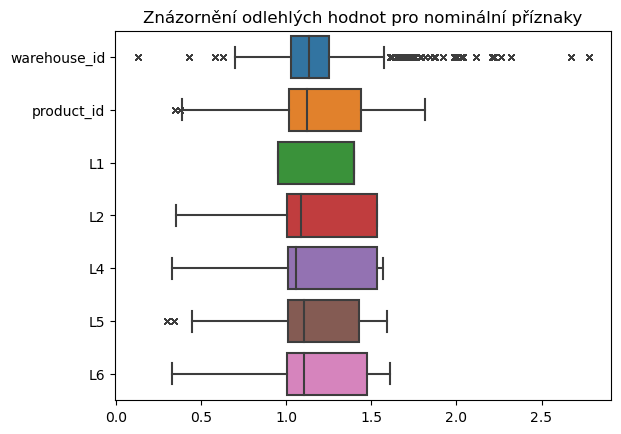
\includegraphics[width=.96\textwidth]{obrazky/zntb/box_nominal.png}
        \caption{Znázornění odlehlých hodnot pro nominální příznaky.}
        \label{obr:rok:g:outlierN}
    \end{minipage}%
    \begin{minipage}{.5\textwidth}
        \centering
        \captionsetup{justification=centering}

        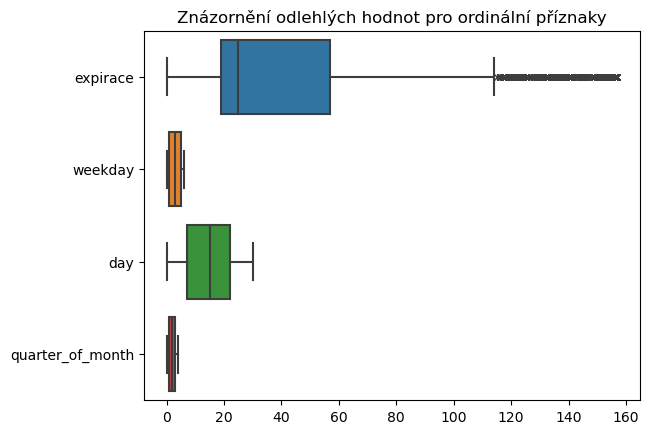
\includegraphics[width=.98\textwidth]{obrazky/zntb/box_ordinal.png}
        \caption{Znázornění odlehlých hodnot pro nominální příznaky.}
        \label{obr:rok:g:outlierO}
    \end{minipage}
\end{figure}

Pomocí Tukeyho testu jsem identifikovala přes $150\ 000$ outlierů pro příznak ID prodejny (\texttt{warehouse\_id}), čímž se dataset zredukoval na $1\ 218\ 453$ řádků. S tímto krokem klesl i počet ostatních outlierů.

V dalším kroku jsem se zaměřila na míru korelace mezi proměnnými. Vizualizovala jsem data pomocí scatter matice pro všechny proměnné, matice je možné vidět na obr. č. \ref*{obr:nb:scatter}. Z této matice můžeme na první pohled vidět, že příznaky odpovídající 4BOX kategorizaci a ID produktu vykazují závislost, což plyne z definice uspořádání této hierarchické kategorizace. V následujících krocích je cílem vybrat tu kategorii, která nejlépe popisuje data ve vztahu k shrinkům.

\begin{figure}[h!]
    \centering
    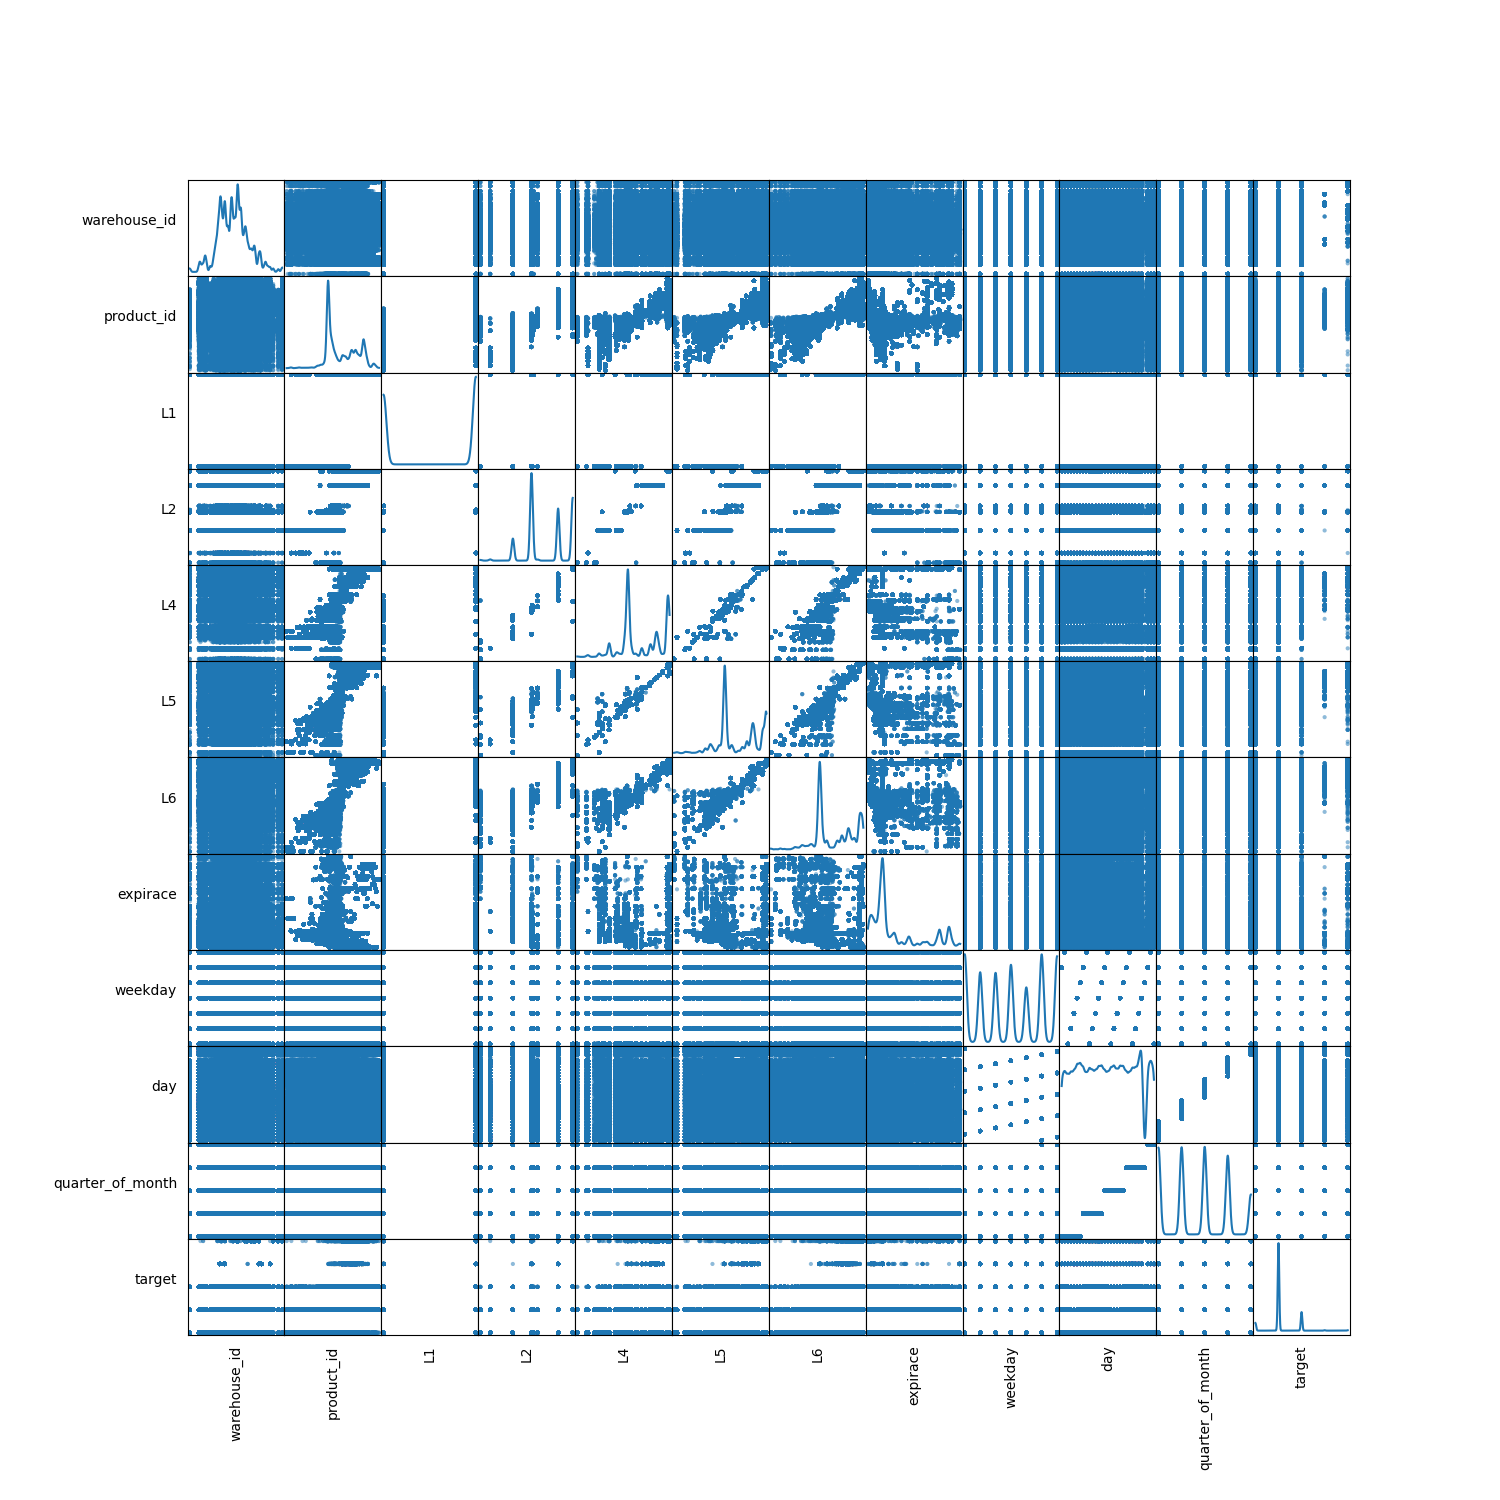
\includegraphics[width=.8\textwidth]{obrazky/zntb/MyScatter.png}
    \caption{Scatter matice příznaků.}
    \label{obr:nb:scatter}
\end{figure}
 
Jako první metodu jsem zvolila $\chi^2$ test. Vzhledem k vysokému počtu dat je matice příliš řídká, a proto nejsou výsledné hodnoty vypovídající a test je tedy pro tuto úlohu nespolehlivý.
Jiným měřítkem pro korelaci mezi proměnnými je Pearsonův korelační koeficient. %!!! odkaz na teorii
Výslednou matici popisující korelační vztahy mezi příznaky jsem vizualizovala teplotní mapou, která je zobrazena na obrázku \ref*{obr:nb:pearson}. Z výsledků je opět patrné, že mezi jednotlivými kategoriemi produktů a produkty je silná korelace. Toto zjištění je zcela logické, neboť se jedná o stromovou strukturu kategorií. Zároveň existuje korelace mezi produktovými kategoriemi a expirací produktu. p-hodnota odpovídající jednotlivým koeficientům byla vždy nulová, kromě pro koeficient týkající se dvojice proměnných expirace a ID prodejny a expirace a pořadí dne v týdnu. Je tedy možné považovat výsledky (kromě těchto dvou výjimek) za statisticky významné.

\begin{figure}[hbtp!]
    \centering
    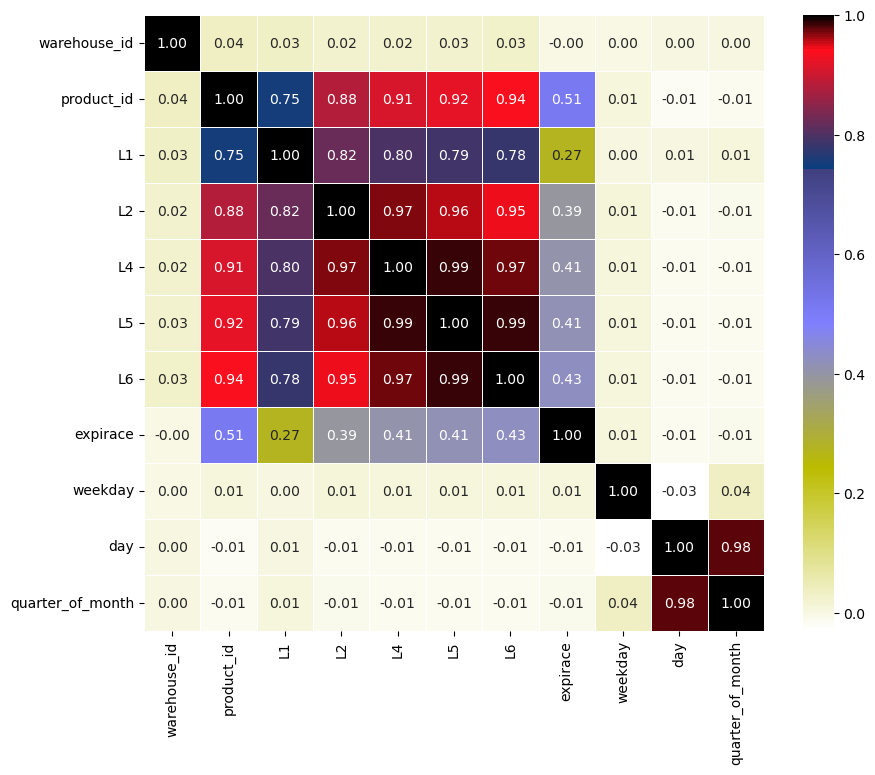
\includegraphics[width=.8\textwidth]{obrazky/zntb/pearson.png}
    \caption{Matice korelačních koeficientů mezi příznaky.}
    \label{obr:nb:pearson}
\end{figure}

Dále jsem použila výpočet koeficientů vzájemné informace \footnote{\emph{mutual information}}, který říká, jaká je podobnost mezi dvěma proměnnými \cite{bib:scikit}. % !!! odkaz na teorii
Matice vypočítaných koeficientů je na obr.\ref*{obr:nb:MI}, jelikož se jedná o symetrickou vlastnost, jsou vynechány hodnoty pod vedlejší diagonálou. Z výsledků je opět vidět zřejmé, že ID produktu sdílí úrovněmi kategorizace tím více, čím je kategorizace jemnější.

\begin{figure}[hbtp!]
    \centering
    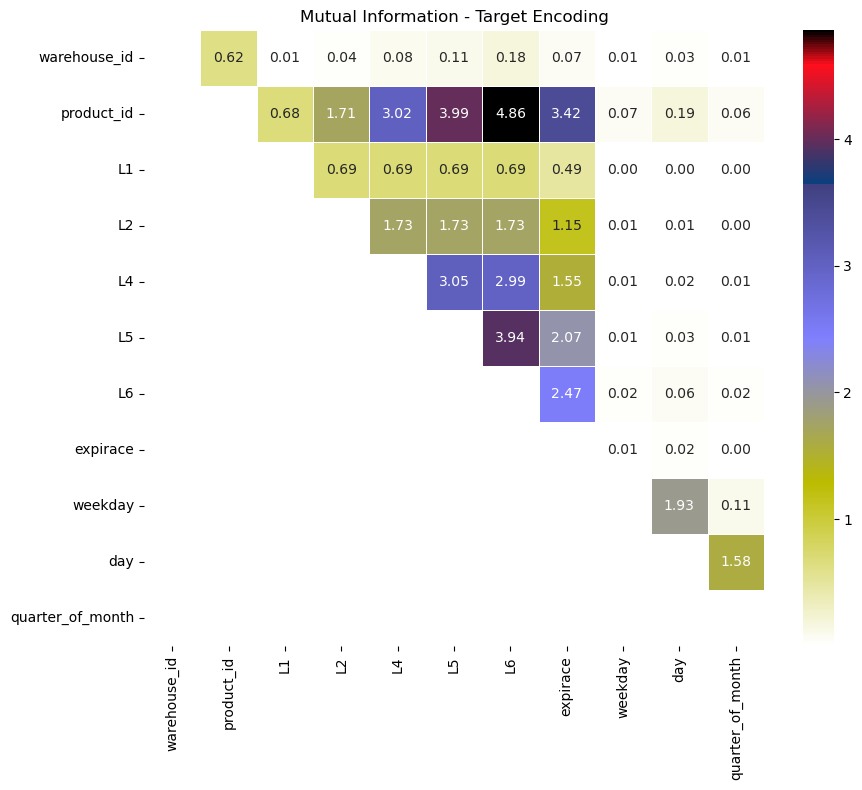
\includegraphics[width=.8\textwidth]{obrazky/zntb/MI_TE.png}
    \caption{Matice koeficientů vzájemné informace mezi příznaky.}
    \label{obr:nb:MI}
\end{figure}

%https://www.statology.org/interpret-cramers-v/
Dále jsem pro znázornění vztahu mezi proměnnými použila koeficient Cramerovo V. Koeficient jsem postupně počítala pro každou dvojici příznaků. Koeficient nabývá hodnot mezi 0 a 1. Číslo blízké nule indikuje, že mezi proměnnými není asociace, číslo blízké jedničce vysokou závislost \cite{bib:statology}. Na obr. \ref*{obr:nb:cramers} lze vidět, že pro kategorie L1 až L6 je hodnota koeficientu  po zaokrouhlení rovna jedné. Vysoká závislost je pak i mezi příznakem expirace a ID produktu a kategorií L1. Dále logicky mezi číslem dne a dnem v týdnu a obdobím v měsíci.
%!!! dopsat co to je %!!!zdroj, odkaz na teorii
\begin{figure}[hbtp!]
    \centering
    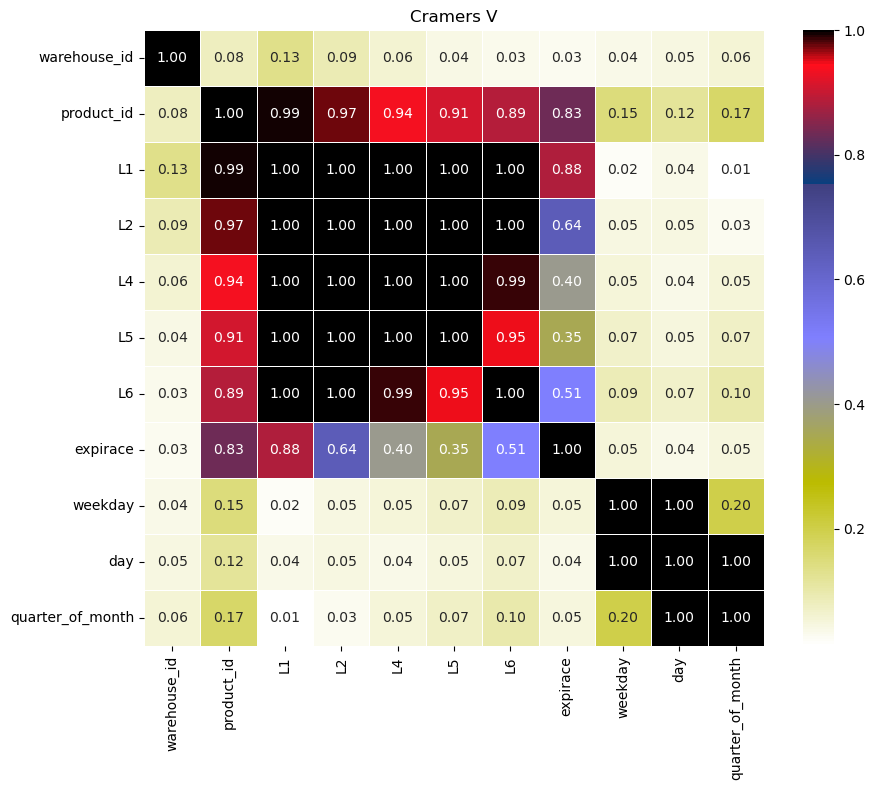
\includegraphics[width=.8\textwidth]{obrazky/zntb/cramers_u.png}
    \caption{Matice koeficientů Cramerovo V mezi příznaky.}
    \label{obr:nb:cramers}
\end{figure}

Další statistikou spočtenou na datech je Theilovo U (neboli koeficient nejistoty), který opět nabývá hodnot mezi 0 a 1 a měří vztah mezi dvěma proměnnými. Na rozdíl od předchozích statistik tento koeficient není symetrický a z výsledků lze vyvodit, ze které proměnné ze dvou zkoumaných můžeme vyvodit informaci o druhé proměnné \cite{bib:correl}. Z výsledků zobrazených v matici na obr. \ref*{obr:nb:thiels} plyne, že z ID produktu lze vyvodit část informace o kategoriích a expiraci. Zatímco úrovně L1 a L2 o ID produktu mnoho informace nenesou. Jak bylo ukázáno i v předchozích statistikách a jak vyplývá z logiky pro získání dne v týdnu a období měsíce, číslo dne nese informaci o těchto dvou příznacích.


\begin{figure}[hbtp!]
    \centering
    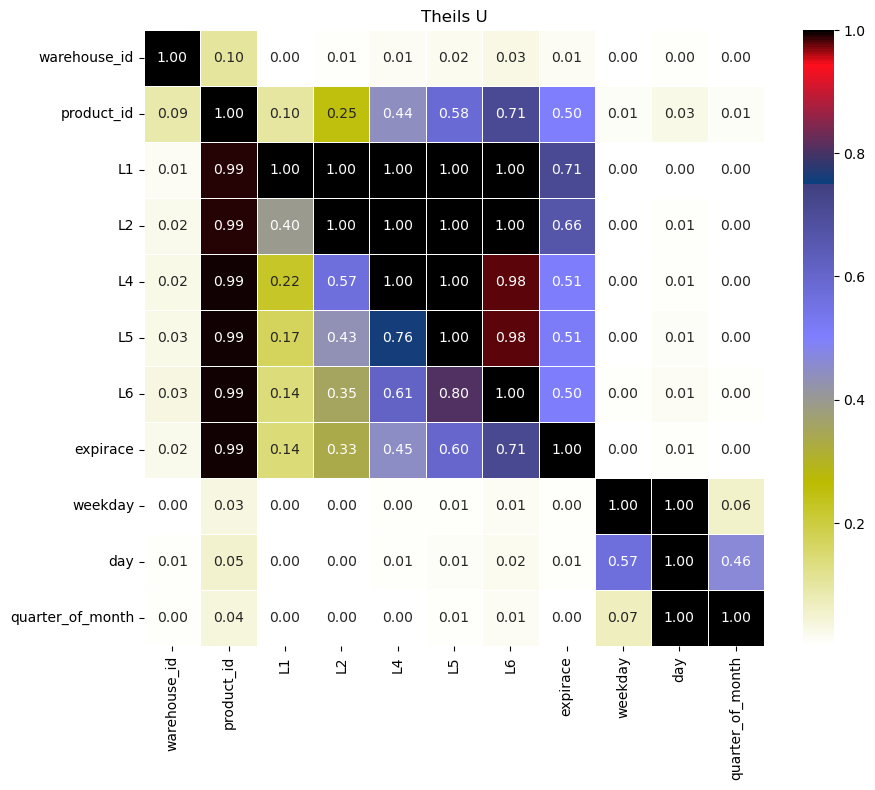
\includegraphics[width=.8\textwidth]{obrazky/zntb/theils_u.png}
    \caption{Matice koeficientů Theilovo U mezi příznaky.}
    \label{obr:nb:thiels}
\end{figure}

Z vypočítaných statistik na datasetu je patrné, že některé příznaky jsou významně závislé, a proto je třeba je z dat odstranit. Kandidáti na vynechání jsou kategorie L2, L4, L6 a číslo dne. V dalších testech budou také vybráni kandidáti a v závěru vyhodnotím, které příznaky byly podle aplikovaných metod vybrány jako vhodné k vynechání a které nikoli.

V dalším testu jsem otestovala multikolinearitu dat pomocí rozptylového inflačního faktoru (VIF). Jako hraniční faktor jsem zvolila hodnotu 40 VIF. Vysvětlující proměnné jsem odebírala z datasetu postupně a odebírání jsem ukončila až, když hodnota VIF nebyla nižší než hraniční.
Tímto došlo k redukci příznaků z jedenácti na pět, a to na kategorii L1, číslo dne, období měsíce, ID prodejny a den v týdnu. Hodnoty koeficientu VIF na datech jsou na obr. \ref*{obr:nb:vif}. 

\begin{figure}[h!]
    \centering
    \begin{minipage}{.5\textwidth}
      \centering
      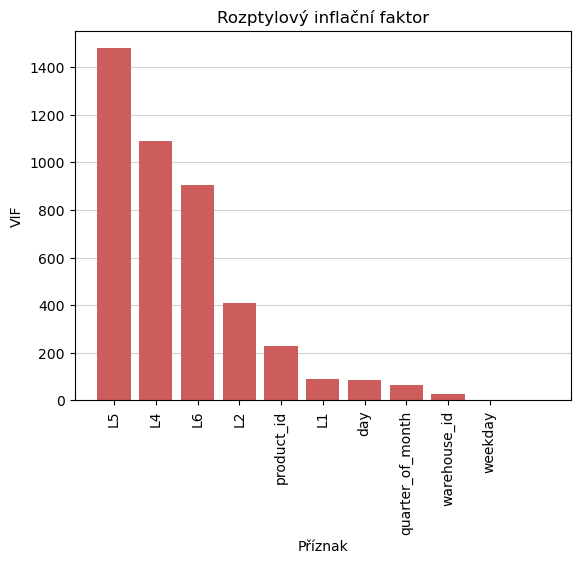
\includegraphics[width=.8\textwidth]{obrazky/zntb/VIF.png}
      \caption{Rozptylový inflační faktor.}
      \label{obr:nb:vif}
    \end{minipage}%
    \begin{minipage}{.5\textwidth}
      \centering
      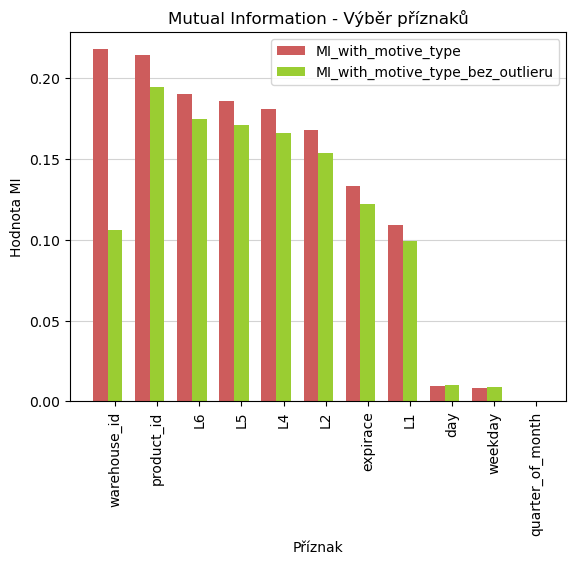
\includegraphics[width=.8\textwidth]{obrazky/zntb/MI_feature_selection.png}
      \caption{Koeficienty vzájemné informace mezi příznaky a cílovým sloupcem typ shrinku.}
      \label{obr:nb:MI_FS}
    \end{minipage}
    \end{figure}

Jako další metodu po výběr příznaků jsem vypočítala hodnotu koeficientů vzájemné informace mezi všemi příznaky s cílovým sloupcem - ID shrinku. Na obrázku \ref*{obr:nb:MI_FS} lze vidět, jak jednotlivé proměnné souvisí s cílovým sloupcem. Pro výpočet tohoto koeficientu jsem použila jak data bez outlierů, tak tenotkrát data před jejich odstraněním. Zde můžeme vidět, že významnost příznaku ID prodejny klesla o téměř polovinu. Nejvíce informace je sdíleno s ID produktu, kategorií L6, dále L5, L4, L2 a expirace. Příznaky související s časovými údaji podle tohoto kritéria nenesou mnoho společné informace.

Jako hlavní metodu pro výběr proměnných jsem se rozhodla použít metodu PCA, tuto metodu je možné použít protože kategorické proměnné jsem převedla na číselné hodnoty v předchozích krocích. Alternativou by bylo použití metody MCA, která se používá pro kategorické datasety, viz dále.
Ve své práci jsem využila implementaci PCA v knihovně \emph{Prince} v jazyce Python. 
Předtím než jsem metodu aplikovala jsem otestovala předpoklad homoskedasticity, tedy shodnost rozptylů v datech, pomocí Bartlettova testu implementovaného v knihovně \emph{factor\_analyzer}. Nulová hypotéza o shodnosti rozptylů nebyla vyvrácena (p-hodnota vyšla nulová). Metodu PCA je proto možné použít.

Na obrázcích \ref*{obr:nb:pca_roztyl_komponetn} a \ref*{obr:nb:pca_kum_roztyl_komponetn} je znázorněno prvních deset komponent a rozptyl který v datech vysvětlují. Na základě hodnot jsem vybrala prvních pět komponent. Již pátá komponenta (označená č. 4) spolu s předchozími vysvětluje více jak 95 \% variability dat. V dalším kroku jsem vypočítala příspěvky příznaků k těmto pěti komponentám a vybrala jsem ty příznaky, které přispívají nejvíce k prvním pěti komponentám. Jejich příspěvek je znázorněný na obr. \ref*{obr:nb:pca_prispevek}. Na základě výsledků analýzy hlavních komponent byly vybrány jako vhodné příznaky pro další práci s daty příznaky - příznaky ID prodejny, den v týdnu, expirace, den a období v měsíci.

\begin{figure}[h!]
    \centering
    \begin{minipage}{.5\textwidth}
      \centering
      \captionsetup{justification=centering}

      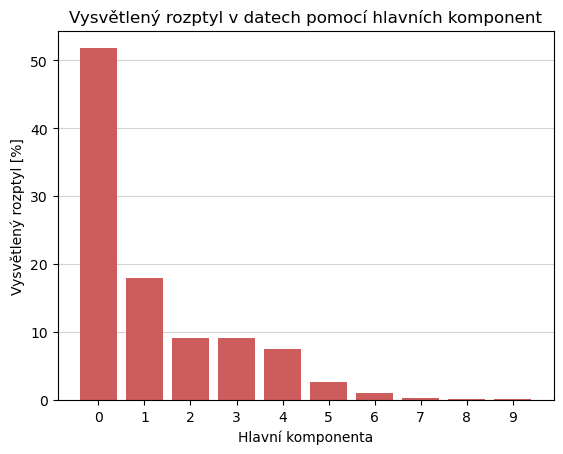
\includegraphics[width=.8\textwidth]{obrazky/zntb/pca-roztyl_komponetn.png}
      \caption{PCA - vysvětlený \\ rozptyl hlavních komponent.}
      \label{obr:nb:pca_roztyl_komponetn}
    \end{minipage}%
    \begin{minipage}{.5\textwidth}
      \centering
      \captionsetup{justification=centering}

      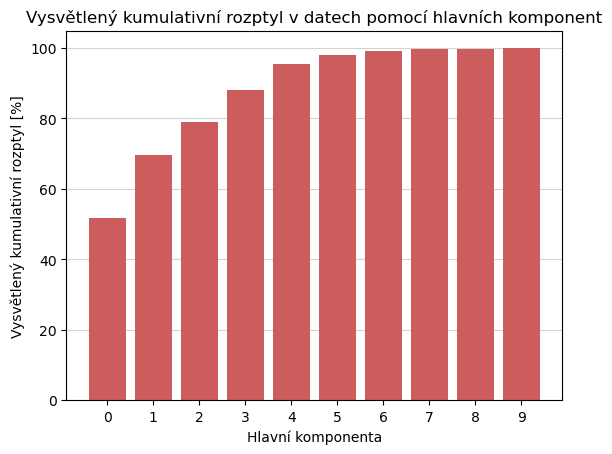
\includegraphics[width=.8\textwidth]{obrazky/zntb/pca-kum_roztyl_komponetn.png}
      \caption{PCA - kumulativní vysvětlený rozptyl hlavních komponent.}
      \label{obr:nb:pca_kum_roztyl_komponetn}
    \end{minipage}
    \end{figure}

\begin{figure}[hbtp!]
    \centering
    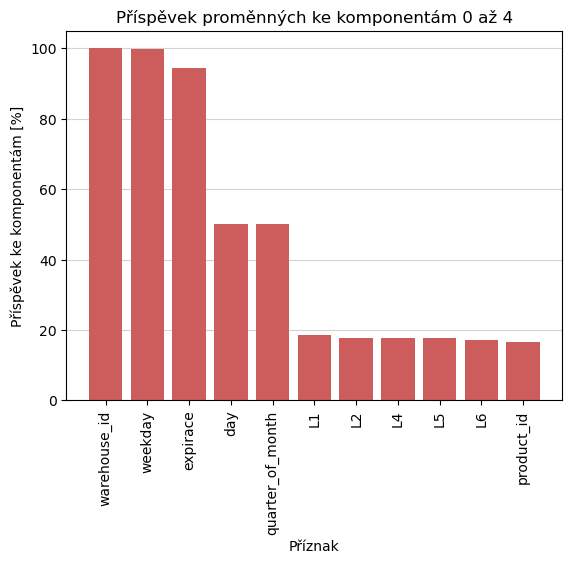
\includegraphics[width=.8\textwidth]{obrazky/zntb/pca-prispevky.png}
    \caption{Příspěvek proměnných ke komponentám 0 až 4.}
    \label{obr:nb:pca_prispevek}
\end{figure}
    
Jak již bylo zmíněno pro redukci dimenzionality u kategorických dat lze použít metodu MCA, opět jsem využila implementaci z knihovny \emph{Prince}. V této implementaci jsou nominální kategorické hodnoty kódovány tak, že narůstá počet sloupců, a proto bylo nutné, vzhledem k nárokům na paměť k uložení matice, omezit množství dat. Vybrala jsem náhodný 20\% vzorek dat, na které jsem MCA aplikovala. Vypočítala jsem prvních pět komponent, které dohromady popisují 79 \% variability dat. Jelikož byla každá kategorie chápána jako samostatná proměnná příspěvky jednotlivých příznaků ke komponentám byly rozmístěny mezi všechny kategorie, nikoli k jednotlivým příznakům. Po agregaci podle původních příznaků největší příspěvek mělo ID produktu, kategorie L6, L5, L4, zatímco nejmenší ID prodejny, L1, den v týdnu a období měsíce. Tyto výsledky je třeba brát se zvážením neboť výpočty probíhali na řádově menším vzorku než u předchozích metod.

% warehouse_id        0.024256
% product_id          1.147270
% L1                  0.035793
% L2                  0.355452
% L4                  0.841652
% L5                  0.911692
% L6                  0.930902
% expirace            0.306007
% weekday             0.035521
% day                 0.362474
% quarter_of_month    0.048981


